%%%%%%%%%%%%%%%%%%%%%%%%%%%%%%%%%%%%%%%%%%%%%%%%%%
%%%%%%%%%%%%%%%%%%%%%%%%%%%%%%%%%%%%%%%%%%%%%%%%%%
%%
%% Last update: 18/09/2019 (English & Chinese Support)
%%
%%%%%%%%%%%%%%%%%%%%%%%%%%%%%%%%%%%%%%%%%%%%%%%%%%
%%%%%%%%%%%%%%%%%%%%%%%%%%%%%%%%%%%%%%%%%%%%%%%%%%
%%
\PassOptionsToPackage{unicode}{hyperref}
\PassOptionsToPackage{naturalnames}{hyperref}
\documentclass{beamer} 
%\usepackage{babel}
%\usepackage[utf8]{inputenc}


%%% FONT SELECTION %%%%%%%%%%%%%%%%%
%%% we choose a sans font %%%%%%%%%%
\usepackage{kmath,kerkis} 
%\usepackage[default]{gfsneohellenic} 
%%%%%%%%%%%%%%%%%%%%%%%%%%%%%%%%%%%%

\usepackage{color}
\usepackage{amsmath}
\usepackage{amssymb}

\usepackage{epstopdf}
\usepackage{graphicx}
\usepackage{IEEEtrantools}
% \usepackage{ctex}
\usepackage{xeCJK}
\setCJKfamilyfont{STSong}{STZhongsong}
\graphicspath{{./images/}}

%%
% load TEI-Pel - specific layout
\usepackage{ecnu}
\setTeipelLayout{red, draft}% options: "draft", "red"
\definecolor{truecolor}{rgb}{0,0.7,0.5}

%%%%%%%%%%%%%%%%%%%%%%%%%%%%%%%%%%%%%%%%%%%%%%%%%%%%%%%%%%%%
% Thesis Info %%%%%%%%%%%%%%%%%%%%%%%%%%%%%%%%%%%%%%%%%%%%%%
%%%%%%%%%%%%%%%%%%%%%%%%%%%%%%%%%%%%%%%%%%%%%%%%%%%%%%%%%%%%
	% title
		\title[基于深度学习的联合实体关系抽取]{基于深度学习的联合实体关系抽取}	
	% author 
    % (In the mandatory argument "{}", separate multiple
    % authors with "\and" - use "\\" for better author name formatting
    % in the title page. In the optional argument "[]" include all
	% author names, with no "\and" or text formatting macros.)
	% Example: 
    %\author[A. Author Albert Einstein]{Anthony Author \and Albert Einstein}
		\author[ChangzhiSun]{孙长志}
	% supervisor	
        \supervisor{指导老师}{孙仕亮}{吴苑斌}
	% date
		\presentationDate{2019年09月18日}
%%%%%%%%%%%%%%%%

\begin{document}

% typeset front slides
	\typesetFrontSlides

%%%%%%%%%%%%%%%%
% Your Slides Start here:

%%%%
\section{实体关系抽取研究背景}
\subsection*{任务介绍}
\begin{frame}{实体关系抽取}

    \begin{figure}[t]
        \begin{center}
            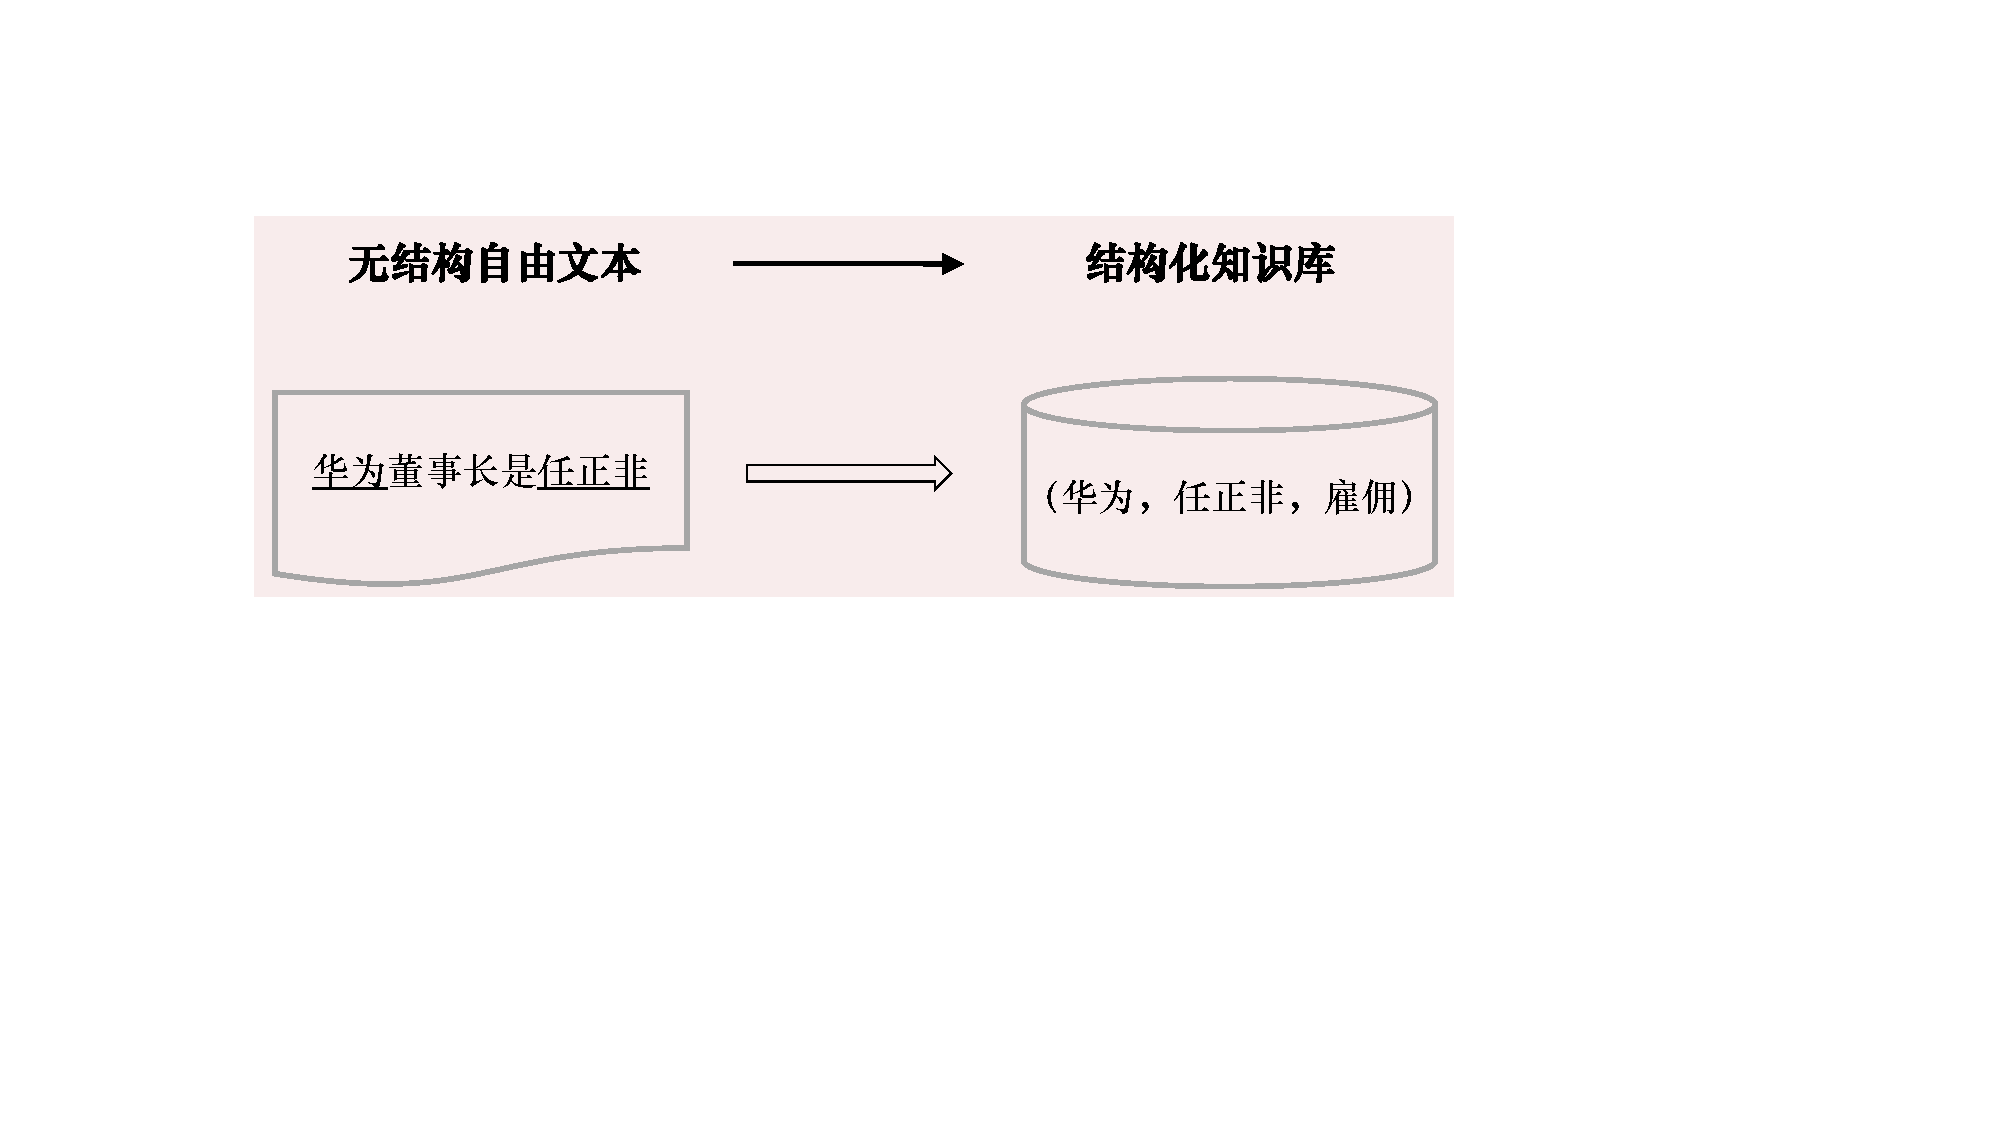
\includegraphics[width=3.5in]{images/task}
        \end{center}
    \end{figure}

	\begin{itemize}
        \item 信息抽取
		\item 实体识别 \& 关系抽取
        \item 为其它任务提供支持
            \begin{itemize}
                \item 知识库填充,自动问答,信息检索 \dots
            \end{itemize}
	\end{itemize}
\end{frame}

\begin{frame}{实体识别}
    \begin{figure}[h]
        \begin{center}
            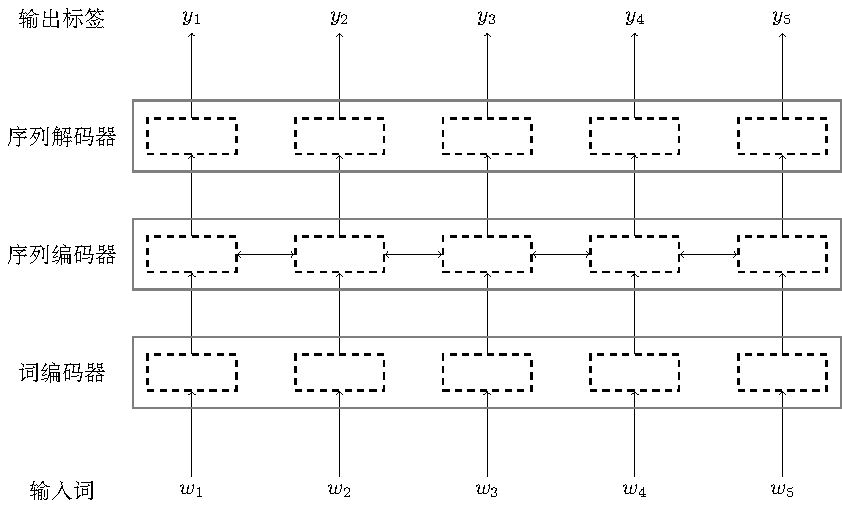
\includegraphics[width=3.5in]{images/seq-label}
        \end{center}
        % \caption{序列标注框架}
    \end{figure}
    \begin{center}
        序列标注框架
    \end{center}

\end{frame}


\begin{frame}{实体识别}
    \begin{itemize}
        \item 词编码器: 离散词 $\rightarrow$ 向量
            \begin{itemize}
                \item 词级别:one-hot 表示,词向量(word2vec,glove)
                \item 字符级别:CNN,biLSTM
                \item 其它特征:词性标注,统计信息
            \end{itemize}
        \item 序列编码器:序列向量$\rightarrow$ 序列向量
            \begin{itemize}
                \item  biLSTM,CNN
            \end{itemize}
        \item 序列解码器:序列向量 $\rightarrow$ 序列离散标签
            \begin{itemize}
                \item  Softmax,CRF
            \end{itemize}
        \item 输出标签:BIO,BILOU
            \begin{figure}[t]
                \begin{center}
                    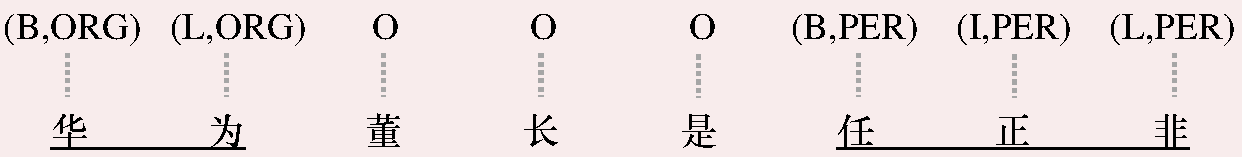
\includegraphics[width=3.9in]{images/entity}
                \end{center}
            \end{figure}
    \end{itemize}
\end{frame}

\begin{frame}{关系抽取}
    \begin{figure}[t]
        \begin{center}
            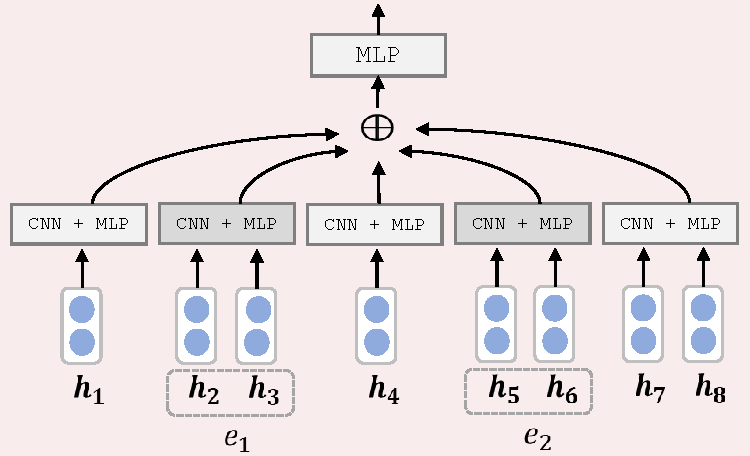
\includegraphics[width=2.8in]{images/relation}
        \end{center}
    \end{figure}

    \begin{itemize}
        \item 多类分类问题 
            \begin{itemize}
                \item 引入 None 关系标签表示没有关系
            \end{itemize}
        \item 特征抽取
            \begin{itemize}
                \item 两个实体特征,实体对上下文特征
            \end{itemize}
    \end{itemize}
\end{frame}

\subsection*{主流方法}
\begin{frame}{主流方法}

	\begin{itemize}
		\item 基于流水线的方法: 两个独立子模型
            \begin{itemize}
                \item \textcolor{truecolor}{ 简单有效}
                \item \textcolor{truecolor}{灵活:易于结合各自的数据集}
                \item \textcolor{red}{错误传播}
            \end{itemize}
        \item 联合模型的方法: 两个子模型统一建模
            \begin{itemize}
                \item \textcolor{truecolor}{利用两个子任务之间的潜在信息,缓解错误传播}
                \item \textcolor{red}{标注数据缺乏}
            \end{itemize}
	\end{itemize}
    \begin{center}
    本文主要研究\textcolor{blue}{联合}实体关系抽取
    \end{center}
\end{frame}

\subsection*{联合模型}
\begin{frame}{联合模型}

	\begin{itemize}
        \item 共享参数: 实体模型和关系模型共享一部分参数 \cite{miwa2016end,katiyar2017going}
            \begin{itemize}
                \item 联合训练
                \item \textcolor{truecolor}{每个子模型可以抽取丰富的特征(没有限制)}
                \item \textcolor{red}{子模型之间的没有显式的交互 (隐式共享参数)}
            \end{itemize}
        \item 联合解码: 更进一步加强两个子模型之间的交互
            \begin{itemize}
                \item \textcolor{truecolor}{可以直接对子模型的输出做约束}
                \item \textcolor{red}{权衡:特征丰富性 \& 解码精确性}
            \end{itemize}
	\end{itemize}
\end{frame}

\begin{frame}{联合解码}

    \begin{itemize}
        \item \textcolor{truecolor}{可以直接对子模型的输出做约束}
        \item \textcolor{red}{权衡:特征丰富性 \& 解码精确性}
            \begin{itemize}
                \item  限制特征 $\rightarrow$ 精确解码 
                    \begin{itemize}
                        \item CRF \cite{katiyar2016investigating}
                        \item 标签扩展\cite{zheng2017joint}
                        \item ILP\cite{yang2013joint}
                    \end{itemize}
                \item  不限制特征 $\rightarrow$ 近似解码 
                    \begin{itemize}
                        \item 全局归一化\cite{zhang2017end}
                        \item 转移系统\cite{wang2018joint}
                        \item 结构化感知机\cite{li2014incremental}
                    \end{itemize}
            \end{itemize}
    \end{itemize}
\end{frame}

%%%%
\section{基于语言学规则的远程监督实体关系抽取}

\section{融合异构数据的实体关系抽取}

\section{基于风险最小化训练的联合实体关系抽取}

\section{基于图卷积网络的联合实体关系抽取}

\section{总结}

\begin{frame}{总结}
    \begin{enumerate}
        \item “数据”
            \begin{itemize}
                \item 基于语言学规则的远程监督实体关系抽取
                \item 融合异构数据的实体关系抽取
            \end{itemize}
        \item “联合模型”
            \begin{itemize}
                \item 基于风险最小化训练的联合实体关系抽取
                \item 基于图卷积网络的联合实体关系抽取
            \end{itemize}
        \item 未来工作
            \begin{itemize}
                \item 预训练
                \item 负样本
            \end{itemize}
    \end{enumerate}
\end{frame}

\section*{}
\begin{frame}
    % \begin{center}
    \Huge{谢谢~ Q\&A}
    % \end{center}
\end{frame}

\section*{参考文献}

\begin{frame}[allowframebreaks]{参考文献}
\bibliographystyle{apalike}
\bibliography{my.bib} % The file containing the bibliography
\end{frame}

%%
\end{document}
